\documentclass{article}
\usepackage[margin=2cm]{geometry}

\usepackage{amsmath}
\usepackage{booktabs} % For table
\usepackage{mathrsfs}
\usepackage{mathtools}
\usepackage{parskip}
\usepackage{bm}
\usepackage{xfrac} % supercedes nicefrac
\usepackage{amsfonts}
\usepackage{setspace}
\usepackage{xr}
\usepackage{pv3rs} % For notation
\usepackage{subcaption} % For subfigure

\newcommand\headercell[1]{% for first row of table
   \smash[b]{\begin{tabular}[t]{@{}c@{}} #1 \end{tabular}}}

% Figures generated by DevFiles/maxima_with_graph_size.R
\title{Ramifications of the prior distribution on relationships graphs}
\date{}
\author{}

\begin{document}
\maketitle

For a given recurrent state, the prior on transitive relationship graphs in uniform. This has various ramifications discussed below. 

\section*{Bounds induced by the prior on the posterior}

When the prior on relapse is non-zero, posterior probabilities of reinfection and recrudescence never reach one because data compatible with either recrudescence or reinfection are also compatible with relapse. In this section we discuss bounds on posterior probabilities of reinfection and recrudescence; they are induced by the uniformity of the prior over transitive relationship graphs. Bounds define a feasible set of posterior probabilities without any information about the genetic data beyond that used to derive the multiplicities of infection. For example, in the case of two genotypes in an enrolment episode followed by a monoclonal recurrence, when recurrent states are equally likely \textit{a priori}, we have $o_{\relap:\reinf} \ge \sfrac{2}{9}$ and $o_{\relap:\recru} \ge \sfrac{4}{9}$. The resulting feasible set of posterior probabilities is shown in Figure~\ref{fig:feasible_set}.

\begin{figure}[h]
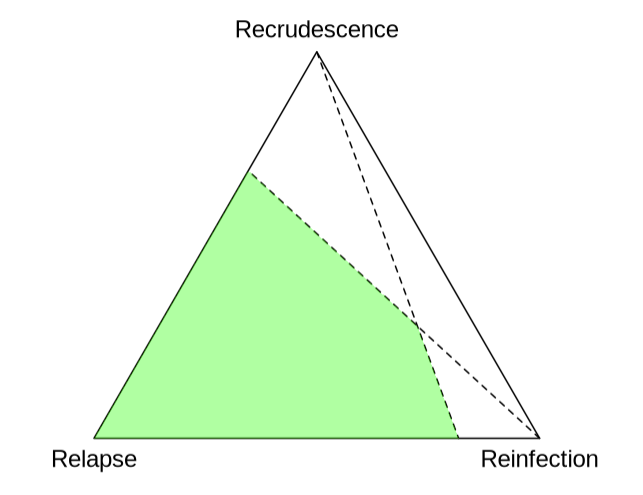
\includegraphics[width=0.5\textwidth]{figures/feasible_moi_2_1.PNG}
\centering
\caption{Feasible set of posterior probabilities in the case of two genotypes in the initial episode and one genotype in the recurrent episode. Dashed lines intersect the left and bottom edges of the simplex at $\frac{4}{9}$ and $\frac{2}{9}$, respectively.}\label{fig:feasible_set}
\end{figure}

\subsection*{How maxima are derived}

We start by making some observations about the posterior odds of relapse to reinfection / recrudescence; odds hold regardless of the posterior probability on the remaining state. 

\subsubsection*{Single recurrence}

For clarity of exposition, we start with the case of a single recurrent episode. Let $\RG_\recru, \RG_\relap,$ and $\RG_\reinf$ denote subsets of the graph space $\RG$, containing the relationship graphs compatible with recrudescence, relapse, and reinfection respectively. The posterior odds of relapse to reinfection is given by

\small
\begin{equation*}
o_{\relap:\reinf} \coloneqq 
\frac{\mathbb{P}(\bm{y} | \relap)\mathbb{P}(\relap)}{\mathbb{P}(\bm{y} | \reinf)\mathbb{P}(\reinf)} =
\frac{\mathbb{P}(\relap)}{\mathbb{P}(\reinf)}
\frac{\sum_{\rg\in\RG_\relap}\mathbb{P}(\bm{y} | \rg)\mathbb{P}(\rg | \relap)}{\sum_{\rg\in\RG_\reinf}\mathbb{P}(\bm{y} | \rg)\mathbb{P}(\rg | \reinf)} =
\frac{\mathbb{P}(\relap)}{\mathbb{P}(\reinf)}
\frac{| \RG_\reinf |}{| \RG_\relap |} \frac{\sum_{\rg\in\RG_\relap}\mathbb{P}(\bm{y} | \rg)}{\sum_{\rg\in\RG_\reinf}\mathbb{P}(\bm{y} | \rg)} = 
\frac{\mathbb{P}(\relap)}{\mathbb{P}(\reinf)}
\frac{| \RG_\reinf |}{| \RG_\relap |} \left(1 + \frac{\sum_{\rg\in\RG_\relap\setminus\RG_\reinf}\mathbb{P}(\bm{y} | \rg)}{\sum_{\rg\in\RG_\reinf}\mathbb{P}(\bm{y} | \rg)}\right), 
\end{equation*}
\normalsize

where $\RG_\relap\setminus\RG_\reinf$ is the subset of graphs compatible with relapse but not reinfection (graphs that have at least one non-stranger inter-episode edge). Similarly, the posterior odds of relapse to recrudescence is given by
\begin{equation*}
o_{\relap:\recru} \coloneqq 
\frac{\mathbb{P}(\bm{y} | \relap)\mathbb{P}(\relap)}{\mathbb{P}(\bm{y} | \recru)\mathbb{P}(\recru)} = 
\frac{\mathbb{P}(\relap)}{\mathbb{P}(\recru)}
\frac{| \RG_\recru |}{| \RG_\relap |} \left(1 + \frac{\sum_{\rg\in\RG_\relap\setminus\RG_\recru}\mathbb{P}(\bm{y} | \rg)}{\sum_{\rg\in\RG_\recru}\mathbb{P}(\bm{y} | \rg)}\right).
\end{equation*}

It follows from these results that 
$o_{\relap:\reinf} \ge 
\sfrac{\mathbb{P}(\relap)| \RG_\reinf |} 
{\mathbb{P}(\reinf)| \RG_\relap |}$ and 
$o_{\relap:\recru} \ge 
\sfrac{\mathbb{P}(\relap)| \RG_\recru |}
{\mathbb{P}(\recru)| \RG_\relap |}$ and that
%
\begin{align} 
\mathbb{P}(\reinf | \bm{y}) &\leq  \label{eq:reinf_prob_max}
\dfrac
{\mathbb{P}(\reinf)}
{\mathbb{P}(\reinf) + 
\mathbb{P}(\relap)\frac{|\RG_\reinf|}{|\RG_\relap|}}, \\
\mathbb{P}(\recru | \bm{y}) &\leq \label{eq:recru_prob_max} 
\dfrac{\mathbb{P}(\recru)}
{\mathbb{P}(\recru) + \mathbb{P}(\relap)
\frac{|\RG_\recru|}{|\RG_\relap|}},  
\end{align}
These inequalities are close to equality when
\begin{itemize}
\item $\sum_{\rg\in\RG_\reinf}\mathbb{P}(\bm{y} | \rg) >> \sum_{\rg\in\RG_\relap\setminus\RG_\reinf}\mathbb{P}(\bm{y} | \rg)$, which implies $\sum_{\rg\in\RG_\recru}\mathbb{P}(\bm{y} | \rg)$ is negligible,
\item $\sum_{\rg\in\RG_\recru}\mathbb{P}(\bm{y} | \rg) >> \sum_{\rg\in\RG_\relap\setminus\RG_\recru}\mathbb{P}(\bm{y} | \rg)$, which implies $\sum_{\rg\in\RG_\reinf}\mathbb{P}(\bm{y} | \rg)$ is negligible. 
\end{itemize}
For example, 
\begin{align*}
 \mathbb{P}(\recru | \bm{y}) 
 &= 
 \dfrac 
 {\sum_{\rg\in\RG_\recru}\mathbb{P}(\bm{y} | \rg)
 \mathbb{P}(\rg | \RG_\recru)\mathbb{P}(\recru)}
 {\sum_{\rg\in\RG_\recru}\mathbb{P}(\bm{y} | \rg)
 \mathbb{P}(\rg | \RG_\recru)\mathbb{P}(\recru) + 
 \sum_{\rg\in\RG_\relap}\mathbb{P}(\bm{y} | \rg)
 \mathbb{P}(\rg | \RG_\relap)\mathbb{P}(\relap) + 
 \sum_{\rg\in\RG_\reinf}\mathbb{P}(\bm{y} | \rg)
 \mathbb{P}(\rg | \RG_\reinf)\mathbb{P}(\reinf)}, \\
 &= 
 \dfrac 
 {\sum_{\rg\in\RG_\recru}\mathbb{P}(\bm{y} | \rg)
 \sfrac{\mathbb{P}(\recru)}{|\RG_\recru|}}
 {\sum_{\rg\in\RG_\recru}\mathbb{P}(\bm{y} | \rg)
 \sfrac{\mathbb{P}(\recru)}{|\RG_\recru|} + 
 \left(\sum_{\rg\in\RG_\recru}\mathbb{P}(\bm{y} | \rg) + 
 \sum_{\rg\in\RG_\relap\setminus\RG_\recru}\mathbb{P}(\bm{y} | \rg)\right) 
 \sfrac{\mathbb{P}(\relap)}{|\RG_\relap|} +
 \sum_{\rg\in\RG_\reinf}\mathbb{P}(\bm{y} | \rg)
 \sfrac{\mathbb{P}(\reinf)}{|\RG_\reinf|}}.
\end{align*}
which simplifies to
$ \mathbb{P}(\recru | \bm{y}) = 
 \mathbb{P}(\recru) \left\{
 {\mathbb{P}(\recru) +  
 \mathbb{P}(\relap)\sfrac{|\RG_\recru|}{|\RG_\relap|}} \right\}^{-1}
$
when $\sum_{\rg\in\RG_\recru}\mathbb{P}(\bm{y} | \rg) >>
\sum_{\rg\in\RG_\relap\setminus\RG_\recru}\mathbb{P}(\bm{y} | \rg)$
because $\sum_{\rg\in\RG_\reinf}\mathbb{P}(\bm{y} | \rg)$ 
is negligible when $\sum_{\rg\in\RG_\recru}\mathbb{P}(\bm{y} | \rg) >> \sum_{\rg\in\RG_\relap\setminus\RG_\recru}\mathbb{P}(\bm{y} | \rg)$. 


\subsubsection*{More than one recurrence}

$$
\frac{p(\bm{y}|\relap X)}{p(\bm{y}|\recru X)} = \frac{\sum_{\rg\in\RG_\relap}\mathbb{P}(\bm{y} | \rg)\mathbb{P}(\rg | \relap X)}{\sum_{\rg\in\RG_\recru}\mathbb{P}(\bm{y} | \rg)\mathbb{P}(\rg | \recru X)}
$$

When there is more than one recurrence and prior probabilities are non-zero, the maximum probabilities of all sequences are non-certain with the exception of the relapse-only sequence. As before, we can compute odds; for example
\begin{align*}
o_{\relap\relap:\recru\relap} \coloneqq
\frac{\mathbb{P}(\bm{y} | \relap\relap)\mathbb{P}(\relap\relap)}{\mathbb{P}(\bm{y} | \recru\relap)\mathbb{P}(\recru\relap)} =
\frac{\mathbb{P}(\relap\relap)}{\mathbb{P}(\recru\relap)}
\frac{| \RG_{\recru\relap} |}{| \RG_{\relap\relap} |} \frac{\sum_{\rg\in\RG_{\relap\relap}}\mathbb{P}(\bm{y} | \rg)}{\sum_{\rg\in\RG_{\recru\relap}}\mathbb{P}(\bm{y} | \rg)} = 
\frac{\mathbb{P}(\relap\relap)}{\mathbb{P}(\recru\relap)}
\frac{| \RG_{\recru\relap} |}{| \RG_{\relap\relap} |} \left(1 + \frac{\sum_{\rg\in\RG_{\relap\relap}\setminus\RG_{\recru\relap}}\mathbb{P}(\bm{y} | \rg)}{\sum_{\rg\in\RG_{\recru\relap}}\mathbb{P}(\bm{y} | \rg)}\right).
\end{align*}
However, unlike before, we cannot always derive maximum posterior probabilities from the odds because the probabilities of the remaining sequences are not necessarily zero when the posterior odds of the relapse-only sequence is minimised (the exception being the odds of all-but-one-relapse to all-relapse sequences). Instead, we must compute maximum probabilities the long way; for example,
\begin{align} 
    \mathbb{P}(\recru\recru | \bm{y}) = 
    &\left\{
    \sum_{\rg\in\RG_{\recru\recru}} \mathbb{P}(\bm{y} | \rg) 
    \sfrac{\mathbb{P}(\recru\recru)}{|\RG_{\recru\recru}|} 
    \right\} \left\{
    \sum_{\rg\in\RG_{\recru\recru}} \mathbb{P}(\bm{y} | \rg) 
    \sfrac{\mathbb{P}(\recru\recru)}{|\RG_{\recru\recru}|}  
    + \left(
    \sum_{\rg\in\RG_{\recru\recru}} \mathbb{P}(\bm{y} | \rg) + 
    \smashoperator{\sum_{\rg\in\RG_{\relap\recru}\setminus\RG_{\recru\recru}}} 
    \mathbb{P}(\bm{y} | \rg)
    \right) \frac{\mathbb{P}(\relap\recru)}{|\RG_{\relap\recru}|}
    \right.  \nonumber \\ 
    + &\left. 
    \left(
    \sum_{\rg\in\RG_{\recru\recru}} \mathbb{P}(\bm{y} | \rg) +
    \smashoperator{\sum_{\rg\in\RG_{\relap\relap}\setminus\RG_{\recru\recru}}}
    \mathbb{P}(\bm{y} | \rg) \right) \frac{\mathbb{P}(\relap\relap)}{|\RG_{\relap\relap}|} 
    + 
    \left(
    \sum_{\rg\in\RG_{\recru\recru}} \mathbb{P}(\bm{y} | \rg) +
    \smashoperator{\sum_{\rg\in\RG_{\recru\relap}\setminus\RG_{\recru\recru}}}
    \mathbb{P}(\bm{y} | \rg) \right) \frac{\mathbb{P}(\recru\relap)}{|\RG_{\recru\relap}|}
    + \sum_{\rg\in\RG_{\recru\reinf}} \mathbb{P}(\bm{y} | \rg) 
    \sfrac{\mathbb{P}(\recru\reinf)}{|\RG_{\recru\reinf}|} +
    \right. \nonumber \\ 
    + &\left. 
    \sum_{\rg\in\RG_{\relap\reinf}} \mathbb{P}(\bm{y} | \rg) 
    \sfrac{\mathbb{P}(\relap\reinf)}{|\RG_{\relap\reinf}|} + 
    \sum_{\rg\in\RG_{\reinf\recru}} \mathbb{P}(\bm{y} | \rg) 
    \sfrac{\mathbb{P}(\reinf\recru)}{|\RG_{\reinf\recru}|} + 
    \sum_{\rg\in\RG_{\reinf\relap}} \mathbb{P}(\bm{y} | \rg) 
    \sfrac{\mathbb{P}(\reinf\relap)}{|\RG_{\reinf\relap}|} + 
    \sum_{\rg\in\RG_{\reinf\reinf}} \mathbb{P}(\bm{y} | \rg) 
    \sfrac{\mathbb{P}(\reinf\reinf)}{|\RG_{\reinf\reinf}|} 
    \right\}^{-1} \label{eq:CC_prob_max}
\end{align}
converges to 
\begin{equation*} 
\dfrac{
\mathbb{P}(\recru\recru)}{
\mathbb{P}(\recru\recru) + 
\mathbb{P}(\relap\recru)\frac{|\RG_{\recru\recru}|}{|\RG_{\relap\recru}|} + 
\mathbb{P}(\relap\relap)\frac{|\RG_{\recru\recru}|}{|\RG_{\relap\relap}|} + 
\mathbb{P}(\recru\relap)\frac{|\RG_{\recru\recru}|}{|\RG_{\recru\relap}|}}  
\end{equation*}
when $\sum_{\rg\in\RG_{\recru\recru}} \mathbb{P}(\bm{y} | \rg)$ exceeds the summation over all other subsets of graph space in equation \eqref{eq:CC_prob_max}. 


\section*{Bounds as indicators of data informativeness}

By comparing estimates of joint probabilities to bounds on joint probabilities, the bounds induced by the prior can be used to answer the question could the probability of my most probable state be higher if I added more data? Note the use of `could' and not `would' here. Comparing estimates of marginal probabilities to bounds on marginal probabilities cannot be used analogously because XXX
  
\section*{Bounds given knowledge of no data}

If there are no data on all recurrences but the first, we can compute a bound on the marginal probability that the first recurrences is a recrudescence / reinfection by summing over all eventualities for the recurrence(s) with missing data. For example, the probability that the first of two recurrences is a recrudescence,
\begin{align*}
    \mathbb{P}(s_1 = \recru | \bm{y}) = 
    &\left\{
    \sum_{\rg\in\RG_{\recru\recru}} \mathbb{P}(\bm{y} | \rg) 
    \sfrac{\mathbb{P}(\recru\recru)}{|\RG_{\recru\recru}|} + 
    \sum_{\rg\in\RG_{\recru\relap}} \mathbb{P}(\bm{y} | \rg) 
    \sfrac{\mathbb{P}(\recru\relap)}{|\RG_{\recru\relap}|} + 
    \sum_{\rg\in\RG_{\recru\reinf}} \mathbb{P}(\bm{y} | \rg) 
    \sfrac{\mathbb{P}(\recru\reinf)}{|\RG_{\recru\reinf}|}
    \right\} \\
    &\left\{
    \sum_{\rg\in\RG_{\recru\recru}} \mathbb{P}(\bm{y} | \rg) 
    \sfrac{\mathbb{P}(\recru\recru)}{|\RG_{\recru\recru}|} + 
    \sum_{\rg\in\RG_{\recru\relap}} \mathbb{P}(\bm{y} | \rg) 
    \sfrac{\mathbb{P}(\recru\relap)}{|\RG_{\recru\relap}|} + 
    \sum_{\rg\in\RG_{\recru\reinf}} \mathbb{P}(\bm{y} | \rg) 
    \sfrac{\mathbb{P}(\recru\reinf)}{|\RG_{\recru\reinf}|} 
    \right. \\ 
    + &\left. 
    \left(
    \sum_{\rg\in\RG_{\recru\recru}} \mathbb{P}(\bm{y} | \rg) + 
    \smashoperator{\sum_{\rg\in\RG_{\relap\recru}\setminus\RG_{\recru\recru}}} 
    \mathbb{P}(\bm{y} | \rg)
    \right) \frac{\mathbb{P}(\relap\recru)}{|\RG_{\relap\recru}|} 
    + 
    \left(
    \sum_{\rg\in\RG_{\recru\relap}} \mathbb{P}(\bm{y} | \rg) +
    \smashoperator{\sum_{\rg\in\RG_{\relap\relap}\setminus\RG_{\recru\relap}}}
    \mathbb{P}(\bm{y} | \rg) \right) \frac{\mathbb{P}(\relap\relap)}{|\RG_{\relap\relap}|} 
    \right. \\ 
    + &\left.   
    \left(
    \sum_{\rg\in\RG_{\recru\reinf}} \mathbb{P}(\bm{y} | \rg) +
    \smashoperator{\sum_{\rg\in\RG_{\relap\reinf}\setminus\RG_{\recru\reinf}}}
    \mathbb{P}(\bm{y} | \rg) \right) \frac{\mathbb{P}(\relap\reinf)}{|\RG_{\relap\reinf}|} + 
    \sum_{\rg\in\RG_{\reinf\recru}} \mathbb{P}(\bm{y} | \rg) 
    \sfrac{\mathbb{P}(\reinf\recru)}{|\RG_{\reinf\recru}|} + 
    \sum_{\rg\in\RG_{\reinf\relap}} \mathbb{P}(\bm{y} | \rg) 
    \sfrac{\mathbb{P}(\reinf\relap)}{|\RG_{\reinf\relap}|} \right.\\
    + &\left.
    \sum_{\rg\in\RG_{\reinf\reinf}} \mathbb{P}(\bm{y} | \rg) 
    \sfrac{\mathbb{P}(\reinf\reinf)}{|\RG_{\reinf\reinf}|} 
    \right\}^{-1}, 
\end{align*}
simplifies to 
\begin{equation} \label{eq:s1_C_prop_max_no_data}
  \dfrac{
\mathbb{P}(\recru\recru) + 
\mathbb{P}(\recru\relap) + 
\mathbb{P}(\recru\reinf)}{
\mathbb{P}(\recru\recru) + 
\mathbb{P}(\recru\relap) + 
\mathbb{P}(\recru\reinf) + 
\mathbb{P}(\relap\recru)\frac{|\RG_{\recru\recru}|}{|\RG_{\relap\recru}|} + 
\mathbb{P}(\relap\relap)\frac{|\RG_{\recru\relap}|}{|\RG_{\relap\relap}|} + 
\mathbb{P}(\relap\reinf)\frac{|\RG_{\recru\reinf}|}{|\RG_{\relap\reinf}|}}  
\end{equation}
when data on the first recurrence support recrudescence but there are no data on the second recurrence because when there are no data on the second recurrence $\sum_{\rg\in\RG_{\recru\recru}} \mathbb{P}(\bm{y} | \rg)= 
\sum_{\rg\in\RG_{\recru\relap}} \mathbb{P}(\bm{y} | \rg)= 
\sum_{\rg\in\RG_{\recru\reinf}} \mathbb{P}(\bm{y} | \rg)$ and because data on the first recurrence support recrudescence
\begin{itemize}
    \item $\sum_{\rg\in\RG_{\recru\recru}} \mathbb{P}(\bm{y} | \rg) >> \sum_{\rg\in\RG_{\relap\recru}\setminus\RG_{\recru\recru}}
    \mathbb{P}(\bm{y} | \rg) \text{ and } \sum_{\rg\in\RG_{\reinf\recru}} \mathbb{P}(\bm{y} | \rg)$
    \item $\sum_{\rg\in\RG_{\recru\relap}} \mathbb{P}(\bm{y} | \rg) >> \sum_{\rg\in\RG_{\relap\relap}\setminus\RG_{\recru\relap}}
    \mathbb{P}(\bm{y} | \rg) \text{ and } \sum_{\rg\in\RG_{\reinf\relap}} \mathbb{P}(\bm{y} | \rg)$
    \item $\sum_{\rg\in\RG_{\recru\reinf}} \mathbb{P}(\bm{y} | \rg) >> \sum_{\rg\in\RG_{\relap\reinf}\setminus\RG_{\recru\reinf}}
    \mathbb{P}(\bm{y} | \rg) \text{ and } \sum_{\rg\in\RG_{\reinf\reinf}} \mathbb{P}(\bm{y} | \rg)$
\end{itemize}
 
\section*{How bounds change with graph size}

%Table~\ref{tab:|GI|/|GL|} shows that the values of $| \RG_\reinf |/| \RG_\relap |$ for different sized  graphs, each with a single recurrence. The values of $| \RG_\reinf |/| \RG_\relap |$ decrease with increasing graph size.  
% \begin{table}[h]
% \centering
% \begin{tabular}{@{} *{6}{c} @{}}
% \headercell{Number of genotypes\\in initial episode} & \multicolumn{5}{c@{}}{Number of genotypes in recurrent episode}\\
% \cmidrule(l){2-6}
% & 1 &  2 & 3 & 4 & 5   \\ 
% \midrule
%    1  & 0.3333 & 0.2222 & 0.1667 & 0.1339 & 0.1123 \\
%    2  & 0.2222 & 0.1026 & 0.0581 & 0.0375 & 0.0263 \\
%    3  & 0.1667 & 0.0581 & 0.0257 & 0.0135 & 0.0080 \\
%    4  & 0.1339 & 0.0375 & 0.0135 & 0.0059 & 0.0030 \\
%    5  & 0.1123 & 0.0263 & 0.0080 & 0.0030 & 0.0013 \\
%  \end{tabular}
%  \caption{Values for $| \RG_\reinf |/| \RG_\relap |$ for various graph sizes.}\label{tab:|GI|/|GL|}
%  \end{table}

\begin{figure}[h]
\begin{subfigure}{.5\textwidth}
  \centering
  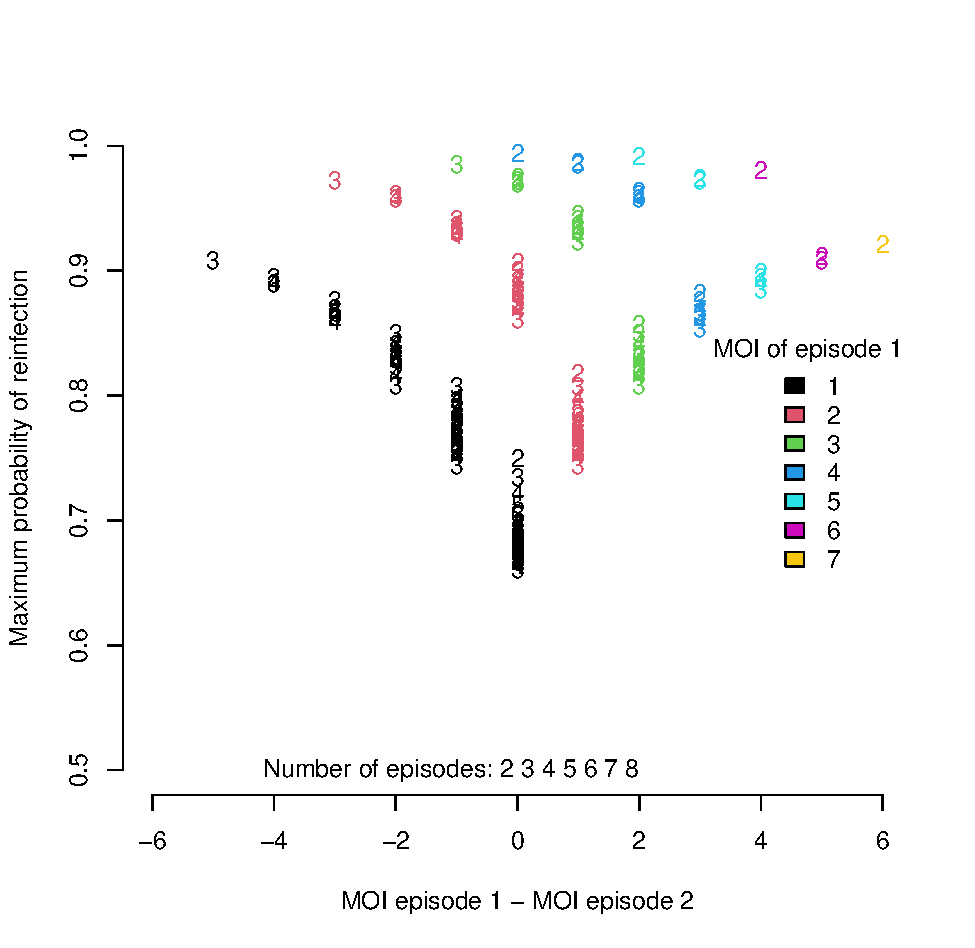
\includegraphics[width=0.9\linewidth]
  {figures/MOIDiff_reinfection.pdf}
  \caption{}
  \label{fig:MOIDiff_reinfection}
\end{subfigure}
\begin{subfigure}{.5\textwidth}
  \centering
  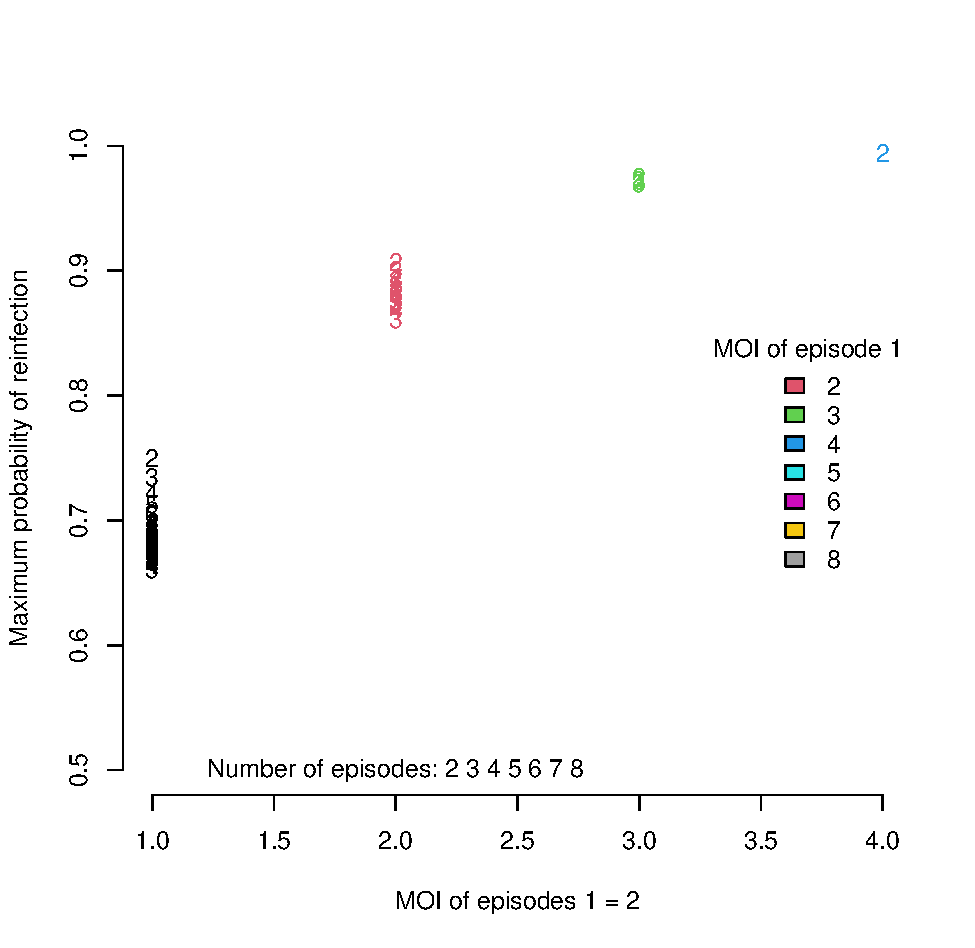
\includegraphics[width=0.9\linewidth]{figures/MOIEqual_reinfection.pdf}
  \caption{}
  \label{fig:MOIEqual_reinfection}
\end{subfigure} \\
\begin{subfigure}{.5\textwidth}
  \centering
  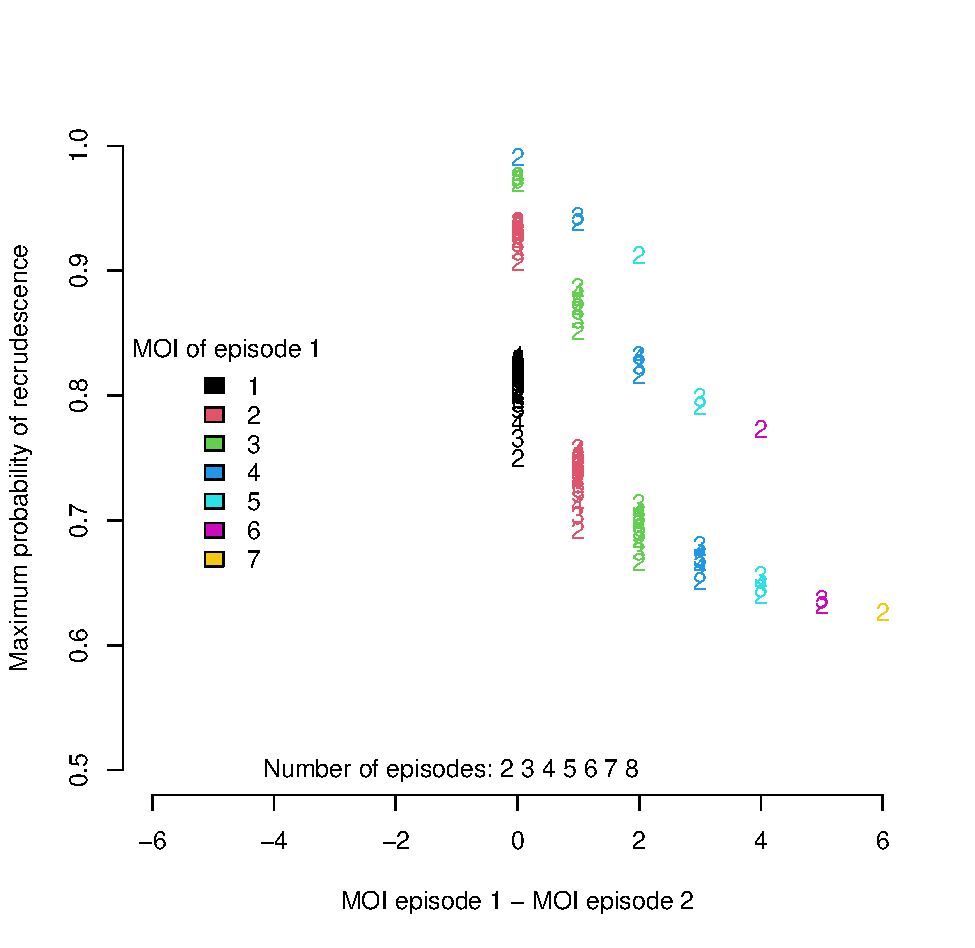
\includegraphics[width=0.9\linewidth]{figures/MOIDiff_recrudescence.pdf}
  \caption{}
  \label{fig:MOIDiff_recrudescence}
\end{subfigure}
\begin{subfigure}{.5\textwidth}
  \centering
  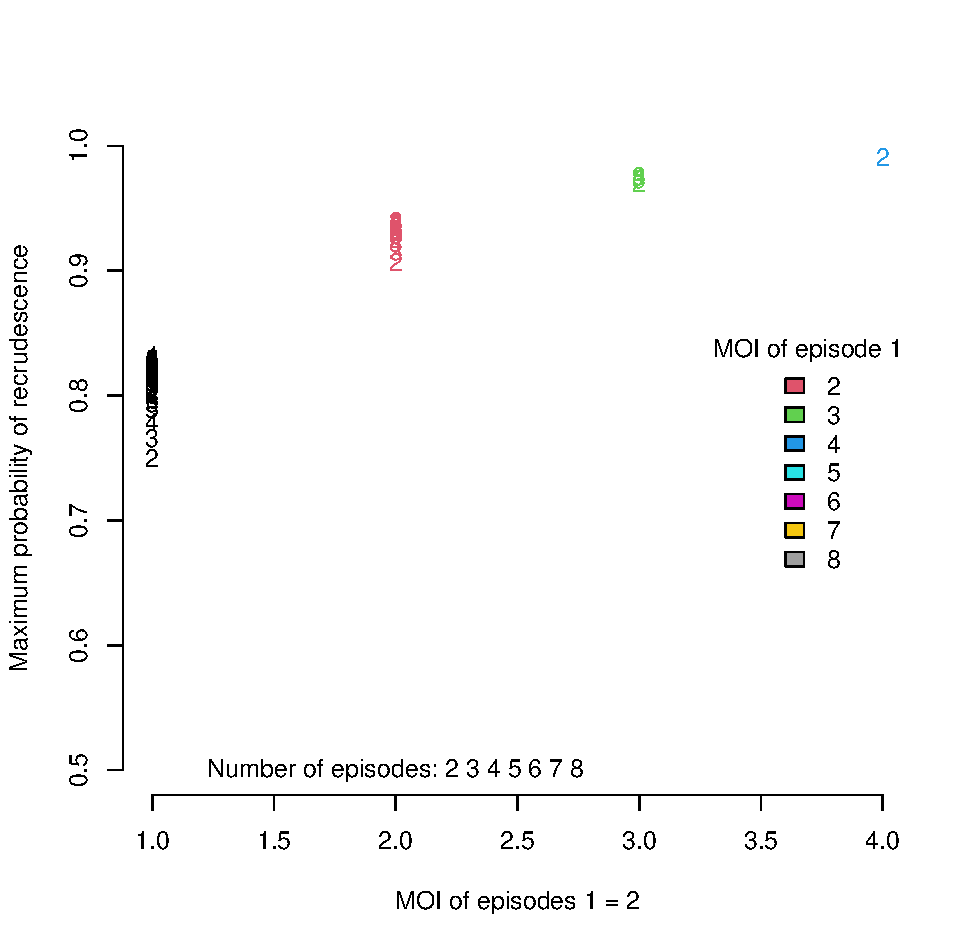
\includegraphics[width=0.9\linewidth]{figures/MOIEqual_recrudescence.pdf}
  \caption{}
  \label{fig:MOIEqual_recrudescence}
\end{subfigure} \\

\caption{Plots of theoretical maximum probabilities of recrudescence and reinfection at the first recurrence in a sequence of two or more episodes. For sequences of only two episodes the maxima are those induced by the prior; for sequences of three or more episodes, maxima are those induced by prior and knowledge of no data on all but the first recurrence (e.g., equation \eqref{eq:s1_C_prop_max_no_data}).}
\label{fig:fig}
\end{figure}

The probability of reinfection increases with the size of the graph, both when MOIs of the enrolment episode are the first recurrence are equal (centre of plot \ref{fig:MOIDiff_reinfection}, detailed in plot\ref{fig:MOIEqual_reinfection}) and not (plot \ref{fig:MOIDiff_reinfection}). The probability of recrudescence increases with graph size when the MOIs of the enrolment episode and the first recurrence are equal (centre of plot \ref{fig:MOIDiff_recrudescence}, detailed in plot \ref{fig:MOIEqual_recrudescence}); it decreases with graph size when MOI of the enrolment episode exceeds that of the first recurrence (when the MOI of recurrence exceeds that of the enrolment episode, recurrence has zero posterior probability); see plot \ref{fig:MOIDiff_recrudescence}. 

\section*{Observations on a counter-intuitive property}

The \textit{a priori} assumption that all valid relationships graphs $\rg$ are equally likely given a recurrent state leads to counter-intuitive properties. Specifically, the probability of an edge can vary depending on the graph it is embedded within. Consider the scenario where one monoclonal recurrence follows a monoclonal enrolment episode. 
%(Example \ref{ex:simplest_het})
Because we assume that the three relationship graphs are equally likely given relapse, the probability distribution of the edge between the two genotypes given relapse is
\begin{align}
    \mathbb{P}(\text{the two genotypes are clones}\vert\bm{s}=\relap) &= \sfrac{1}{3},
    \label{eq: 1st two C gvn L}\\
    \mathbb{P}(\text{the two genotypes are siblings}\vert\bm{s}=\relap) &= \sfrac{1}{3},\\
    \mathbb{P}(\text{the two genotypes are strangers}\vert\bm{s}=\relap) &= \sfrac{1}{3}. 
\end{align}
Now consider the scenario in which there is an additional monoclonal recurrence. 
%(Example \ref{ex:multiple_recurs_het}). 
There are now 12 relationship graphs, which are assumed to be equally likely under relapses. Among them, between the first two genotypes, three have a clonal edge, four have a sibling edge, and five have a stranger edge. The probability distribution of the edge between the first two genotypes given relapses is thus
\begin{align}
    \mathbb{P}(\text{the first two genotypes are clones}\vert\bm{s}=\relap\relap) &= \sfrac{3}{12},
    \label{eq: 1st two C gvn LL}\\
    \mathbb{P}(\text{the first two genotypes are siblings}\vert\bm{s}=\relap\relap) &= \sfrac{4}{12},\\
    \mathbb{P}(\text{the first two genotypes are strangers}\vert\bm{s}=\relap\relap) &= \sfrac{5}{12}.
\end{align}

An explanation for the change in the probability distribution of the edge between the first two genotypes upon the addition of the second relapse is that a clonal edge between the first two genotypes imposes a constraint where the two remaining edges must exhibit the same relationship. Similarly, a sibling edge between the first two genotypes is incompatible with a single stranger edge among the two remaining edges. In general, the pattern that stranger edges are more likely \textit{a priori} and clonal edges are less likely \textit{a priori} becomes more prominent when more genotypes are present. For monoclonal episodes, this change in distribution over the edge between the first two genotypes results in an increase (decrease) in the conditional upper bound (the bound induced by the prior plus knowledge that data are missing for all recurrences beyond the first) on the probability that the first recurrence is a recrudescence (reinfection) with the addition of monoclonal recurrences devoid of data (Figure \ref{fig:monoclonal_recurrences}). 

\begin{figure}
    \centering
    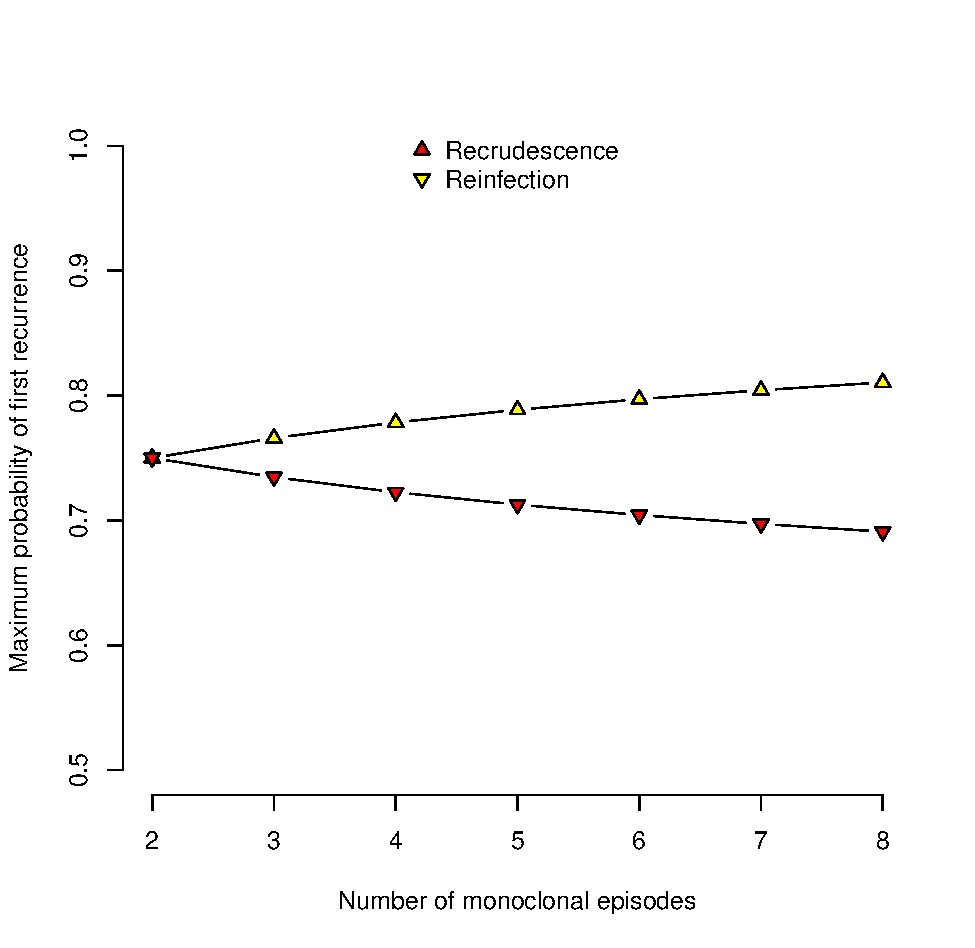
\includegraphics[width=0.8\linewidth]{figures/monoclonal.pdf}
    \caption{The probability that the first recurrence is a recrudescence (reinfection) increases (decreases) with additional recurrences devoid of data. The prior on recurrent states is uniform. The maximum probability is that induced by the prior plus knowledge that all data are missing for recurrences beyond the first. For example, from equations \eqref{eq: 1st two C gvn L} and \eqref{eq: 1st two C gvn LL} we have $\sfrac{|\RG_\recru|}{|\RG_\relap|} = \sfrac{1}{3} > \sfrac{|\RG_{\recru\relap}|}{|\RG_{\relap\relap}|} = \sfrac{3}{12}$. Plugging $\sfrac{|\RG_\recru|}{|\RG_\relap|} = \sfrac{1}{3}$ into equation \eqref{eq:recru_prob_max}, and $\sfrac{|\RG_{\recru\relap}|}{|\RG_{\relap\relap}|} = \sfrac{3}{12}$ plus $\sfrac{|\RG_{\recru\recru}|}{|\RG_{\relap\recru}|} = \sfrac{1}{3}$ and $\sfrac{|\RG_{\recru\reinf}|}{|\RG_{\relap\reinf}|} = \sfrac{1}{3}$ into equation \eqref{eq:s1_C_prop_max_no_data}, we see that the probability that the first recurrence is a recrudescence when recurrent states are equally likely \textit{a priori} increases slightly from $\sfrac{3}{4}$ to $\sfrac{3}{\left(3 + \sfrac{11}{12}\right)}$ with the addition of the second recurrence without data. If we add yet another recurrence, the first recurrence is elevated further.}
    \label{fig:monoclonal_recurrences}
\end{figure}

Consider a second example of a counter-intuitive property induced by the uniformity of the prior over transitive relationship graphs, this time with multiple genotypes per episode. Suppose that there is a reinfection episode with MOI one after an initial episode with MOI $M\ge 2$. Since we have a reinfection, all inter-episode edges must be stranger edges. The number of valid relationship graphs is the $M$-th Bell number $B_M$, since each relationship graph is equivalent to partitioning the genotypes in the initial episode by sibling relationships. We now consider the probability that the first two genotypes in the initial episode are siblings. The number of relationship graphs where the first two genotypes are siblings is $B_{M-1}$, since we can ignore one of the first two genotypes for enumeration purposes. Thus, the probability that the first two genotypes are siblings is $\sfrac{B_{M-1}}{B_M}$, which is asymptotically $\mathcal{O}(1/M)$ as $M\rightarrow\infty$. Arguably, this probability should not vanish as $M\rightarrow\infty$, at least not for a single inoculation of many parasite. (For $M\rightarrow\infty$ with the number of bites $n_b\rightarrow\infty$, the overall proportion of sibling comparisons might approach zero but at a different rate: for example, if on average a mosquito co-transmits $n_s$ siblings among $n_p$ parasites per bite and $M$ increases with the number of bites $n_b$, we could argue the overall proportion of sibling comparisons within an infection should be $\sfrac{\left(n_b \binom{n_p}{2} \right)}{\binom{n_b n_p}{2}}$.)

The impact of the distribution on a given edge changing with its environment evidently varies with the number of genotypes; e.g., in Figure \ref{fig:monoclonal_recurrences}, where data are missing for all recurrences but the first, the impact dwindles. Presumably, its impact on the posterior when data are not missing also varies with the number of genotypes. However, its impact on the posterior in a data-rich setting is hard to ascertain. 

%Copied comments
%Jan 24, 2025 8:15 AM 
%ysfoo: 1. When there is a lot of information in the data, the unintended features of a uniform RG distribution can be drowned out. Recall the likelihood sum p(data|3Rs) = sum of p(data|RG)*p(RG|3Rs) over RG. For the example I wrote in this doc, the fact that p(first pair is X|LL) is different for different X was my "unintended feature". Yet this does not matter for the vignette example because p(data|an RG where first pair are clones) dominates any p(data|an RG where first pair are not clones), given the 100 matching rare alleles. So the feature that clones are less favoured in a uniform RG distribution did not matter here.


\end{document}